
\documentclass[a4paper]{article}
\usepackage[pdftex]{graphicx}
\usepackage[utf8]{inputenc}
\usepackage{enumerate}
\usepackage{icomma}
\usepackage{siunitx}
\sisetup{locale=DE} 
\usepackage{amssymb}
\usepackage{tikz}
\usepackage{href-ul}
\hypersetup{
	colorlinks=true,
	linkcolor=blue,
	urlcolor=blue}
\usepackage{geometry}
\geometry{a4paper, top=15mm, left=15mm, right=15mm, bottom=15mm,
	headsep=10mm, footskip=12mm}
%Source: img_0217

% Start the document
\begin{document}
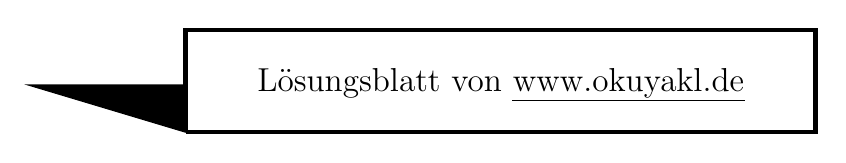
\begin{tikzpicture}(10,3)
	\draw[ultra thick](2,0) --(10,0) -- (10,1.3) --(2,1.3) -- (2,0);
	\draw[fill=black](2,0)-- (0,.6) -- (2,.6) -- (2,0);
	\node at (6,.6) {\large Lösungsblatt von \href{https://www.okuyakl.de}{www.okuyakl.de}};
\end{tikzpicture}
\vspace{0.5 cm}

L Ö S U N G 

\noindent{\bf Aufgabe 1.}\\
Wir berechnen zunächst das Volumen einer solchen Kugel:
$$V={4\over 3}\pi r^3 = {4\over 3}\pi \cdot(\SI{1}{\meter})^3 =\SI{4,19}{\meter}^3$$
$1000~dm^3 = \SI{1}{\meter}^3 \quad \Rightarrow \quad \SI{1}{\meter}^3$ wiegt $\SI{30}{\kilogram} \quad \Rightarrow$ die Kugel wiegt:
$$m_K=\SI{4,19}{\meter}^3\cdot \SI{30}{\kilogram\per\meter^3}=\SI{126}{\kilogram}$$
Man kann diese Kugel nicht alleine tragen; sie ist zu schwer (und zu unhandlich).

\noindent{\bf Aufgabe 2.}\\
Durch Umstellen der Formel für das Kugelvolumen erhalten wir für den Radius:
$$
\renewcommand{\arraystretch}{2}
\begin{array}{rcll}
V &=& {4 \over 3} \pi r^3 & | \cdot {3 \over 4 \pi}\\
{3 V\over 4 \pi}&=& r^3 &|\sqrt[3]{\quad}\\
\sqrt[3]{3 V\over 4 \pi}&=& r &={d\over 2}\\
d&=& 2\cdot \sqrt[3]{3 V\over 4 \pi} &(*)
\end{array}
$$
\noindent{\bf Aufgabe 2.a)}\\
Wir setzen $V=\SI{1}{\meter}^3$ in $(*)$ ein:
$$d= 2\cdot \sqrt[3]{3\cdot \SI{1}{\meter}^3 \over 4 \pi}= \SI{1,24}{\meter}$$

\noindent{\bf Aufgabe 2.b)}\\
Wir setzen $V=\SI{49}{\centi\meter}^3$ in $(*)$ ein:
$$d= 2\cdot \sqrt[3]{3\cdot \SI{49}{\centi\meter}^3 \over 4 \pi}= \SI{4,54}{\centi\meter}$$

\noindent{\bf Aufgabe 3.}\\
Die Dose hat die Höhe $h=6r$. Das Zylindervolumen ist damit:
$$ V_Z = \pi r^2 \cdot h= 6\pi r^3$$
Das Volumen der drei Bälle ist:
$$V_{3B} = 3\cdot  {4 \over 3} \pi r^3 = 4 \pi r^3 $$
Das Volumen der Zwischenräume ist die Differenz davon; der prozentuale Anteil am Zylindervolumen errechnet sich mit der Formel:
$$p\% = \left({V_{Z}-V_{3B} \over V_{Z}}\right)\cdot 100\% = \left(1-{V_{3B} \over V_{Z}}\right)\cdot 100\% = \left(1- {4\pi r^3 \over 6 \pi r^3}\right)\cdot 100\% = \left(1-{4\over 6}\right)\cdot 100\% = 33\%$$

\noindent{\bf Aufgabe 4.}\\
Wir nehmen das Kugelvolumen als Referenz und setzen nacheinander das Zylinder- und das Kegelvolumen damit gleich und lösen nach der jeweiligen Höhe $h$ auf.\\
Höhe des Zylinders:
$$
\renewcommand{\arraystretch}{2}
\begin{array}{rcll}
V_K &=& V_Z \\
{4 \over 3} \pi r^3 &=& \pi r^2 \cdot h_Z &|: \pi r^2\\
 {4 \over 3} r &=& h_Z\\
\end{array}
$$
Höhe des Kegels:
$$
\renewcommand{\arraystretch}{2}
\begin{array}{rcll}
V_K &=& V_{Ke} \\
{4 \over 3} \pi r^3 &=& {1\over 3} \pi r^2 \cdot h_{Ke} &|: {1\over 3} \pi r^2\\
4 r &=& h_{Ke}\\
\end{array}
$$
Vergleicht man die Höhe dieser drei Körper, so ist der Zylinder am niedrigsten, die Kugel mit der Höhe $2r$ ist an zweiter Stelle, am höchsten ist der Kegel.

\noindent{\bf Aufgabe 5.}\\
Das Volumen eines Tropfens ist:
$$V_T={4 \over 3} \pi (\SI{2}{\milli\meter})^3 =\SI{33,5}{\milli\meter}^3$$
Die Anzahl der Tropfen in einer Woche ist bei 30 Tropfen pro Minute:
$$n=7\cdot 24 \cdot 60 \cdot 30 = 302400$$
Die Wassermenge, die verloren geht, errechnet sich mit der Tropfenanzahl mal des Tropfenvolumens:
$$V = n \cdot V_T = 302400 \cdot \SI{33,5}{\milli\meter}^3 \approx \SI{1e7}{\milli\meter}^3 = \SI{10}{\deci\meter}^3 = 10~l$$

\noindent{\bf Aufgabe 6.}\\
Der Radius $r$ nimmt um ein Zehntel zu und ist dann $1,1~r$. Die prozentuale Zunahme des Volumens errechnet sich dann mit der Formel:
$$\left({V_{neu} \over V_{alt}}-1\right) \cdot 100\% =  \left({{4\over 3} \pi (1,1r)^3 \over {4\over 3} \pi r^3}-1 \right)\cdot 100\% = 
\left({1,1^3 \over 1}-1\right)\cdot 100\% = (1,331-1)\cdot 100\% = 33\%$$

\noindent{\bf Aufgabe 7.}\\
Der Radius der Kugel sei $r$, ihr Volumen $V_K$. Die Kantenlänge des Würfels ist dann $2r$, das Würfelvolumen ist $V_W=(2r)^3=8r^3$.
Der prozentuale Anteil des Volumens der einbeschriebenen Kugel ist folglich:
$${V_K \over V_W}\cdot 100\% = {{4 \over 3} \pi r^3 \over 8 r^3}= {{4 \over 3} \pi \over 8} \cdot 100\% = 52\%$$

\noindent{\bf Aufgabe 8. a)}\\
Die Erdoberfläche beträgt insgesamt:
$$ O_E= 4\pi r^2 = 4 \pi \cdot (\SI{6370}{\kilo\meter})^2=\SI{5,1e8}{\kilo\meter}^2$$
Das Wasser wäre über diese Fläche gleichmäßig verteilt; Die Wassertiefe $h_E$ wäre hierbei:
$$V = O_E \cdot h_E \quad \Rightarrow \quad h_E = {V\over O_E} = {\SI{1,4e9}{\kilo\meter}^3 \over \SI{5,1e8}{\kilo\meter}^2 }= \SI{2,7}{\kilo\meter} $$

\noindent{\bf Aufgabe 8. b)}\\
Der Oberflächeninhalt des Mondes Europa ist:
$$O_M= 4\pi r^2 = 4 \pi \cdot (\SI{1560}{\kilo\meter})^2=\SI{3,1e7}{\kilo\meter}^2$$
Die Durchschnittliche  Wassertiefe $h_M$ ist hierbei:
$$V = O_E \cdot h_M \quad \Rightarrow \quad h_M = {V\over O_M} = {2 \cdot \SI{1,4e9}{\kilo\meter}^3 \over \SI{3,1e7}{\kilo\meter}^2 }= \SI{90}{\kilo\meter} $$

\noindent{\bf Aufgabe 9. a)}\\
Das Volumen beider Kugeln mit dem Radius $1,5a$ ist gleich dem Volumen der vereinigten Kugel mit dem neuen Radius $R$. Wir setzen beide Volumina gleich und lösen nach dem neuen Radius auf: 
$$
\renewcommand{\arraystretch}{2}
\begin{array}{rcll}
2\cdot {4 \over 3} \pi (1,5~a)^3 &=& {4\over 3} \pi R^3  &|: {4\over 3} \pi \\
2\cdot (1,5~a)^3 &=&  R^3  &|\sqrt[3]{\quad}\\
 \sqrt[3]{2}\cdot 1,5~a&=& R\\
R&=& 1,89~a 
\end{array}
$$
 
\noindent{\bf Aufgabe 9. b)}\\
Die Oberfläche der zwei Kugeln ist:
$$O_{2K} = 2\cdot 4\pi \cdot (1,5~a)^2 = 56,5~a^2$$
Die neue Oberfläche der vereinigten Kugel ist:
$$O_{neu} = 4\pi \cdot (1,89~a)^2 = 44,9~a^2$$
Den prozentualen Anteil der neuen Oberfläche im Vergleich zur alten erhalten wir mit:
$$ {O_{neu} \over O_{2K}} \cdot 100\% = 79,4\%$$

\noindent{\bf Aufgabe 10.}\\
Der Radius der Orange ohne Schale ist 
$$r = {\SI{8,0}{\centi\meter}\over 2} -\SI{0,6}{\centi\meter} = \SI{3,4}{\centi\meter}$$ Das Volumen des Fruchtfleisches ist damit:
$$V= {4 \over 3} \pi \cdot (\SI{3,4}{\centi\meter})^3 = \SI{165}{\centi\meter}^3 = \SI{165}{\milli\liter}$$
Der Saftanteil hiervon beträgt 70\%; multipliziert mit 5 Orangen ergibt dies ein Saftmenge von:
$$V_{ges}=\SI{165}{\milli\liter}\cdot 0,7 \cdot 5 =\SI{576}{\milli\liter}$$

\noindent{\bf Aufgabe 11. a)}\\
Es gilt $$r={\SI{4,27}{\centi\meter} \over 2}=\SI{2,135}{\centi\meter} $$
Damit erhalten wir für die Oberfläche:
$$O= 4\cdot \pi r^2= \SI{57,28}{\centi\meter}^2$$
Und für das Volumen:
$$V={4\over 3} \pi r^3=\SI{40,76}{\centi\meter}^3$$
\noindent{\bf Aufgabe 11. b)}\\
$$ \textnormal{Dichte}\, \varrho = { \textnormal{Masse}\,m \over \textnormal{Volumen} \, V }=
{\SI{45,9}{\gram} \over \SI{40,76}{\centi\meter}^3} = \SI{1,13 }{\gram \per \centi\meter^3} $$
Die Dichte von Wasser ist geringer: $\varrho_{Wasser}=\SI{1}{\gram \per \centi\meter^3} $.\\
\noindent{\bf Aufgabe 11. c)}\\
Der Golfball geht im See unter; er kann nicht schwimmen. [Im Toten Meer $\varrho=\SI{1,24}{\gram \per \centi\meter^3}$ könnte er schwimmen.]

\begin{center}
	\includegraphics[width=7 cm]{../../viecher/endcomic.pdf}
	
	Hier geht es zurück zum \href{https://www.okuyakl.de/math/m10kuvolL217/aa217.pdf}{Aufgabenblatt}
\end{center}

\end{document}
